\documentclass[12pt,a4j,draft]{jsarticle}
\usepackage[margin=15mm]{geometry}
\usepackage[dvipdfmx, final]{graphicx}
\usepackage{here}
\begin{document}

\centerline{
\Large{中間報告書}
}
\rightline{2020年11月19日}
\rightline{B4 佐々一心}


\section{実施内容}
mnistデータセットを用いてMishとTanexpの論文に記述されていたモデルと同じハイパーパラメータでモデルを実装しました。活性化関数のみを変化させて各エポック数ごとの訓練データの損失、精度と検証データの損失、精度を比較しました。比較した活性化関数はrelu, selu(swish), mish, tanexpの4種類の他にreluの簡易的な連続近似のsoftplus、swishに近く、入力が負の時に出力が0に収束しないelu、flatten-Tで提案されていた関数に近いreluから定数を引いた関数(おそらく提案されていない関数)を使用しました。

\section{結果}
モデルの定義はMishとTanexpの論文に記述されていたモデルを使用し、下図の12の全結合層から構成されるBlock層で使用される活性化関数を変化させて比較しました。

\begin{figure}[H]
  \begin{center}
    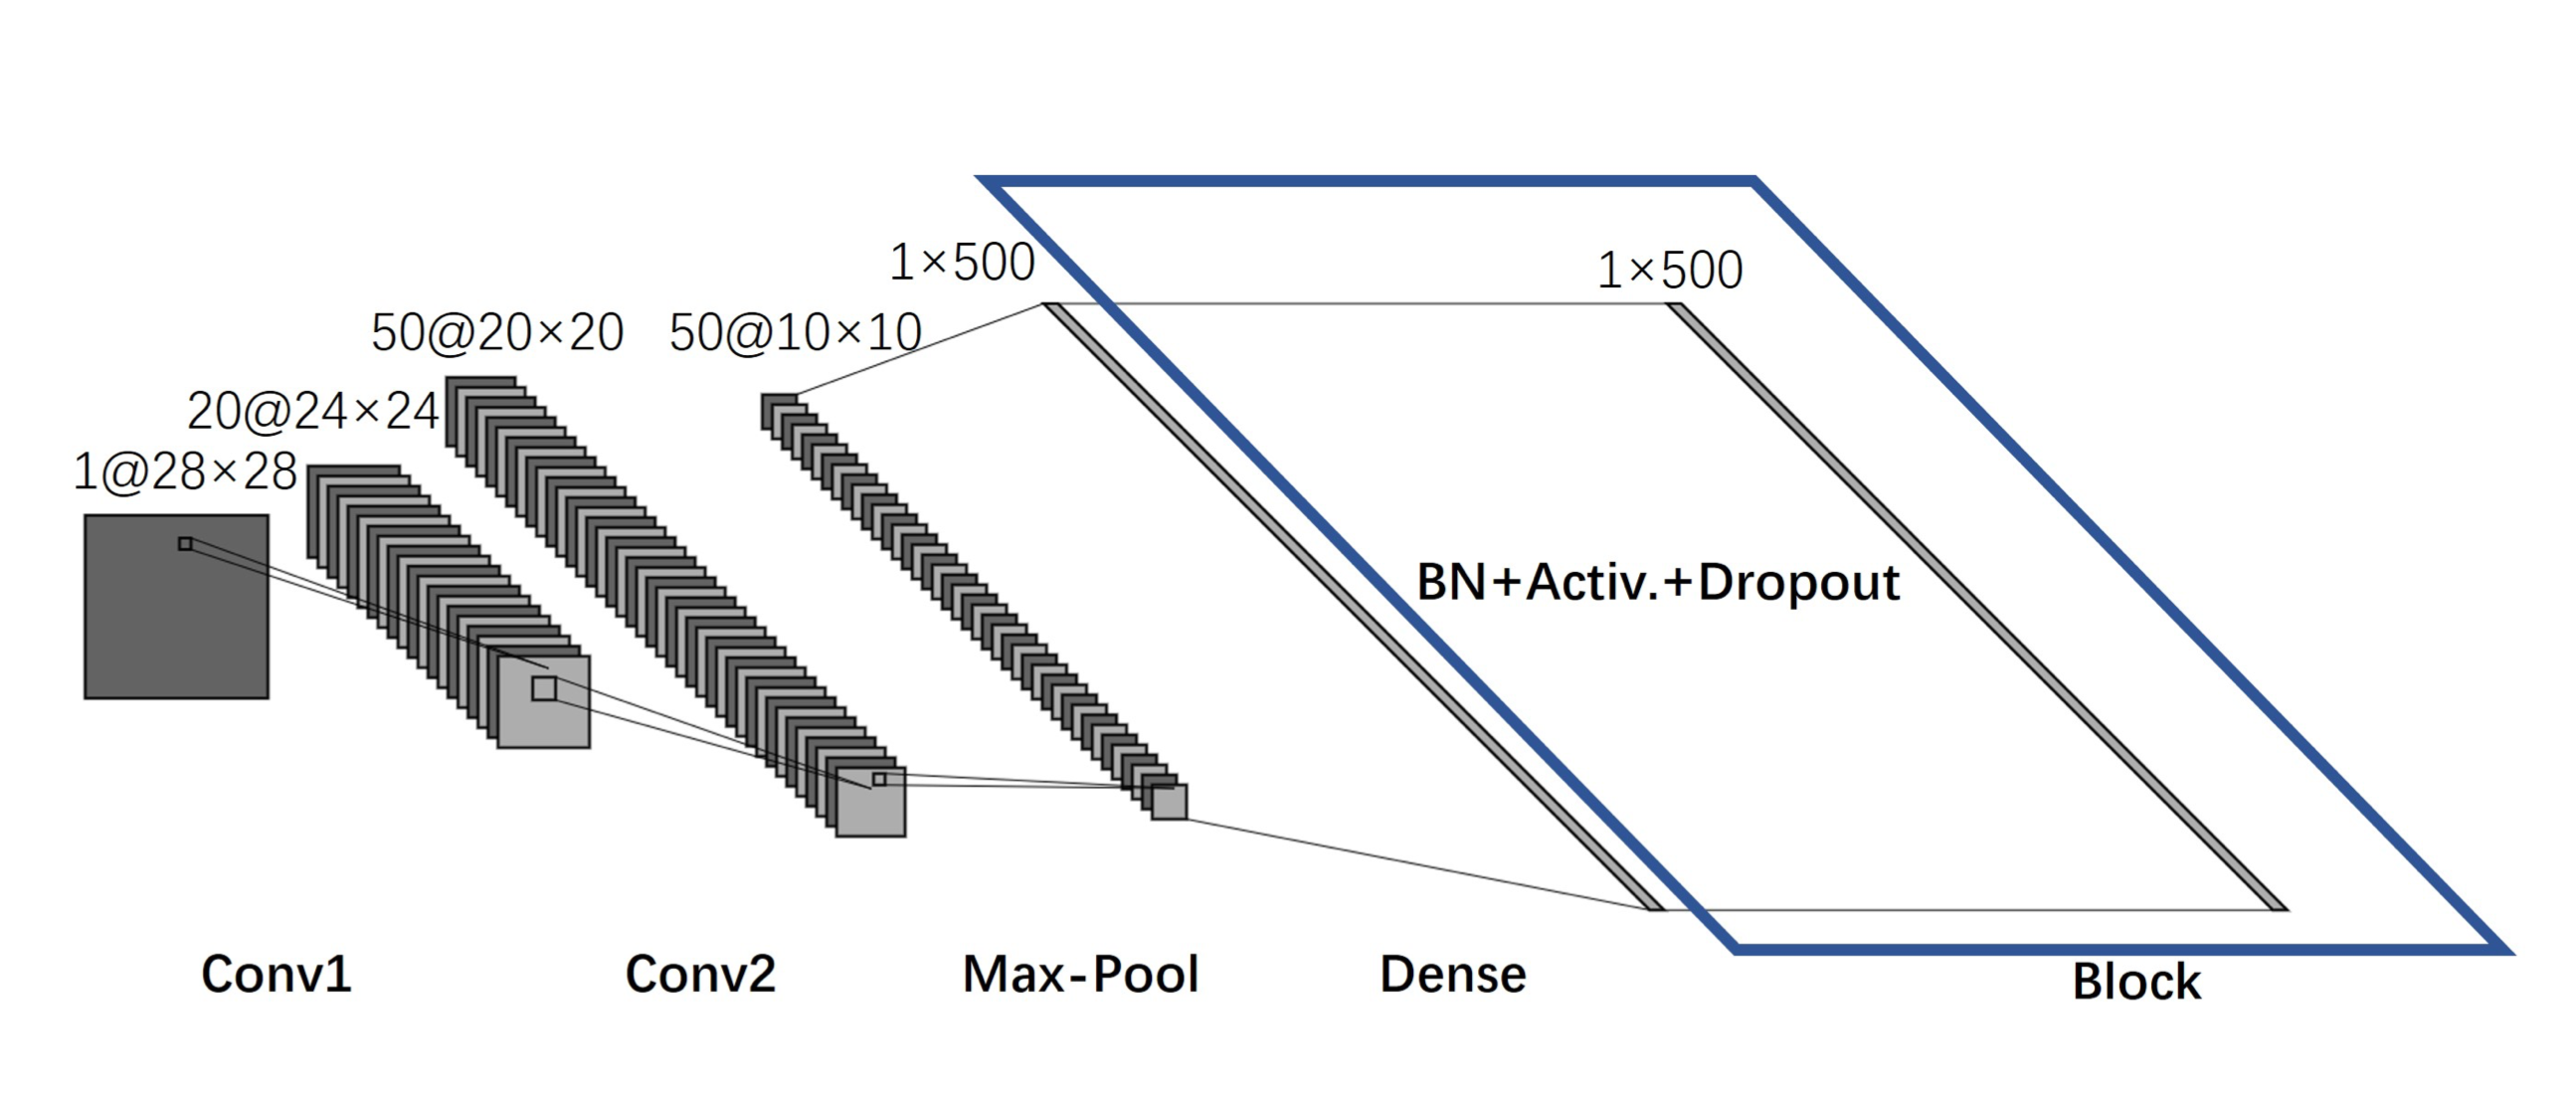
\includegraphics[width=10.0cm]{../image/model.png}
    \caption{使用したモデル}
    \label{model}
  \end{center}
\end{figure}

各エポックごとの精度と損失を比較した結果、最も収束が早く、精度がよかった活性化関数はselu(swish)でした。さらに次いでeluがseluと同等の収束速度、精度でした。10エポックまでの最終精度で比較するとmishが最も高い精度であった。
\begin{table}[H]
 \caption{10エポック目での最終精度}
 \label{10_acc}
 \centering
  \begin{tabular}{cccccccc}
   \hline
   &relu&selu&mish&tanexp&softplus&elu&myopinion \\
   \hline
   accuray&0.9509&0.9793&0.9808&0.9786&0.7298&0.9791&0.9718 \\
   \hline
  \end{tabular}
\end{table}


\begin{figure}[H]
  \begin{center}
    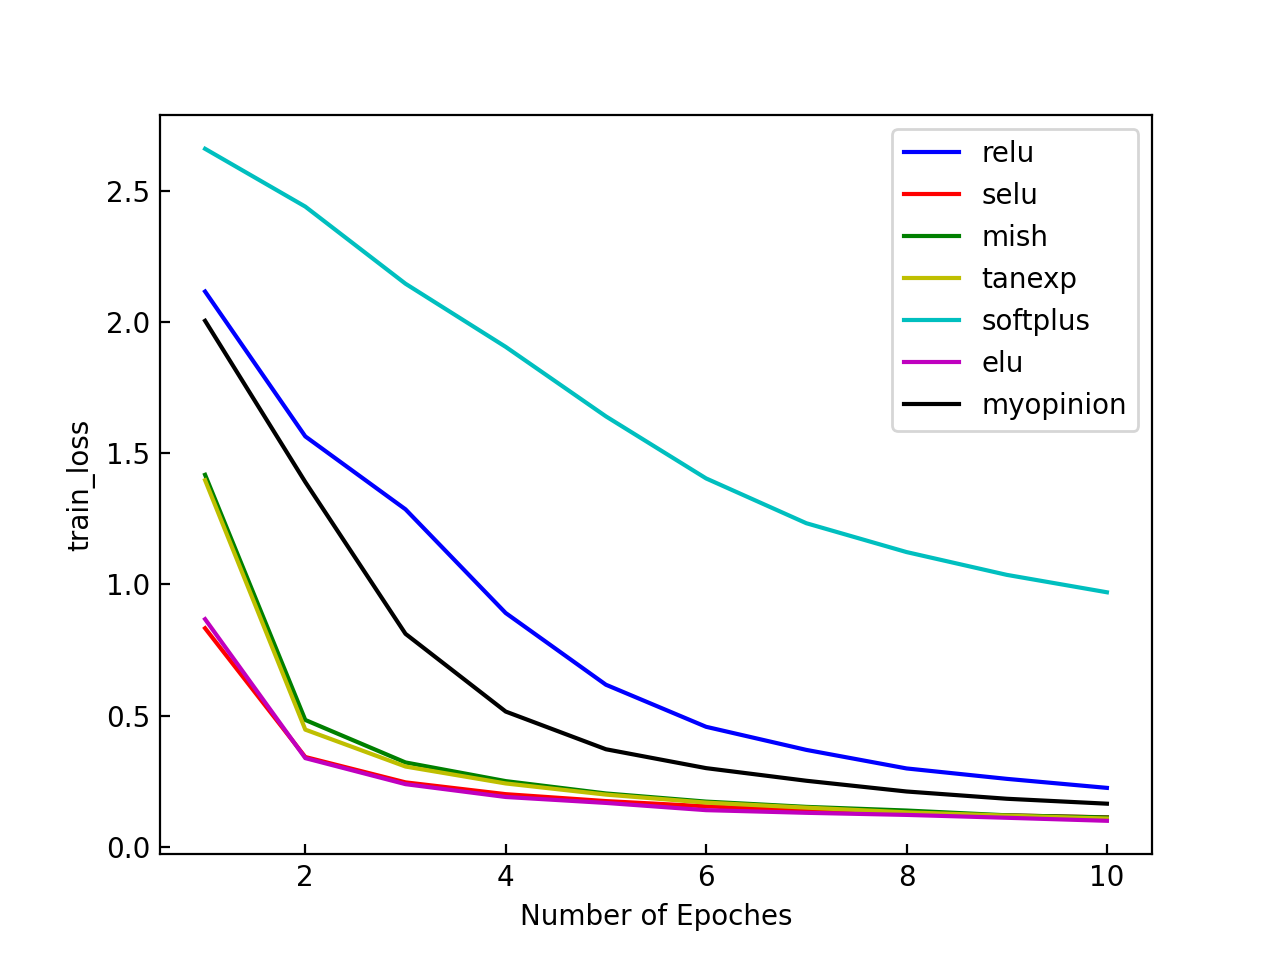
\includegraphics[width=10.0cm]{../comparison_data/mnist_train_loss.png}
    \caption{訓練データでの損失}
    \label{train_loss}
  \end{center}
\end{figure}
\begin{figure}[H]
  \begin{center}
    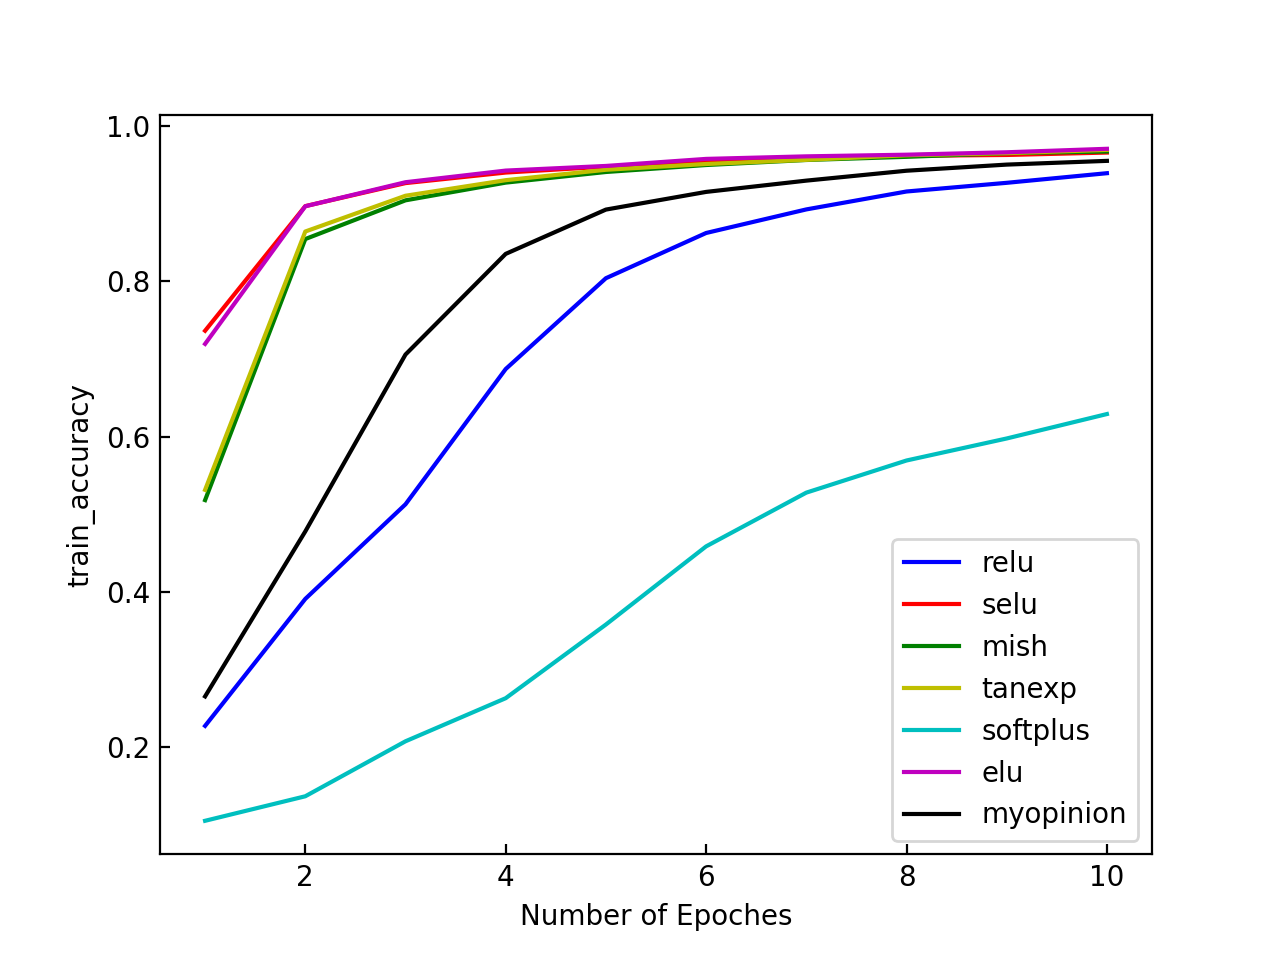
\includegraphics[width=10.0cm]{../comparison_data/mnist_train_acc.png}
    \caption{訓練データでの精度}
    \label{train_acc}
  \end{center}
\end{figure}
\begin{figure}[H]
  \begin{center}
    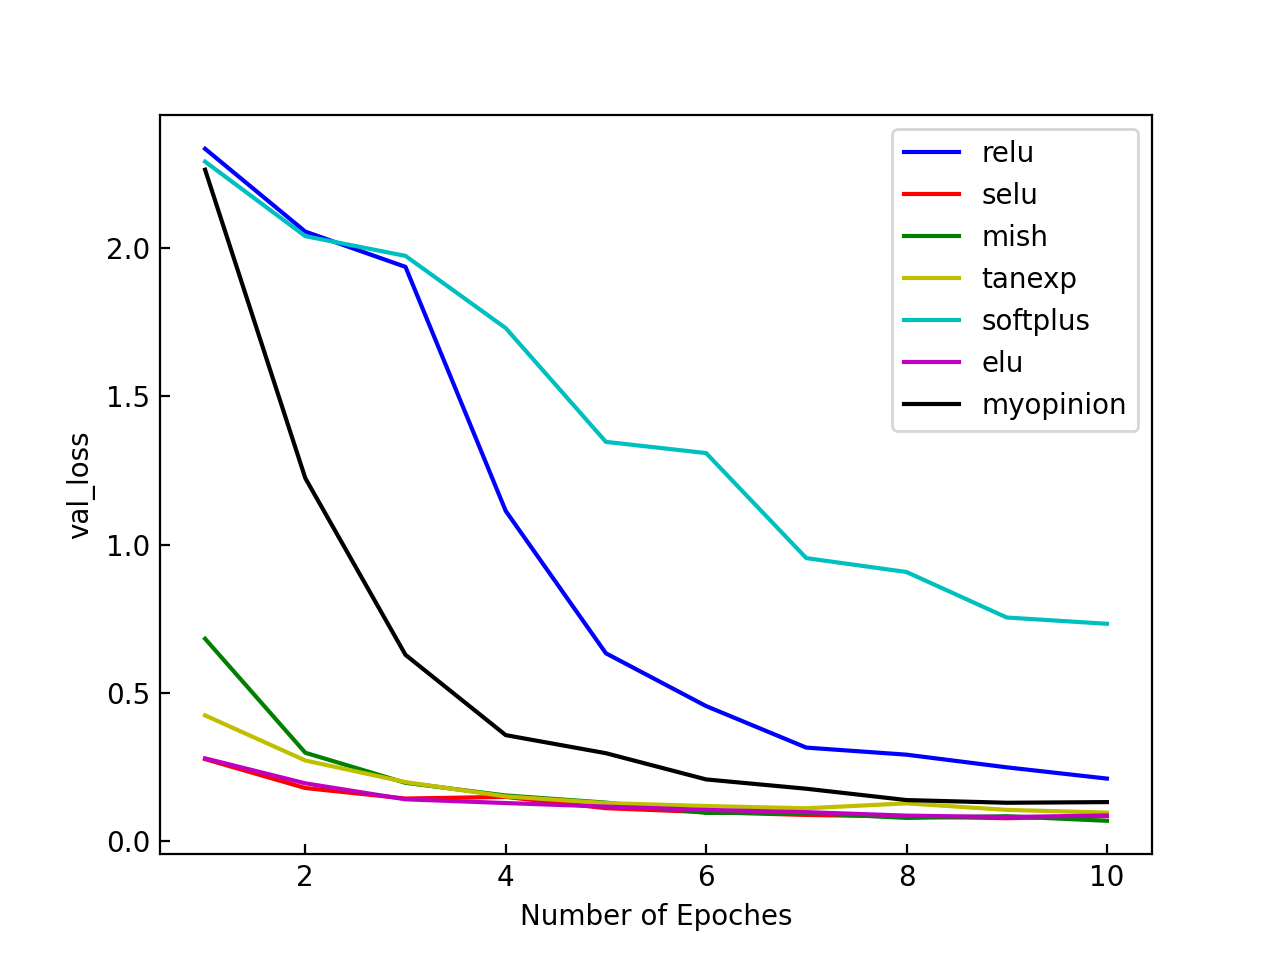
\includegraphics[width=10.0cm]{../comparison_data/mnist_val_loss.png}
    \caption{検証データでの損失}
    \label{val_loss}
  \end{center}
\end{figure}
\begin{figure}[H]
  \begin{center}
    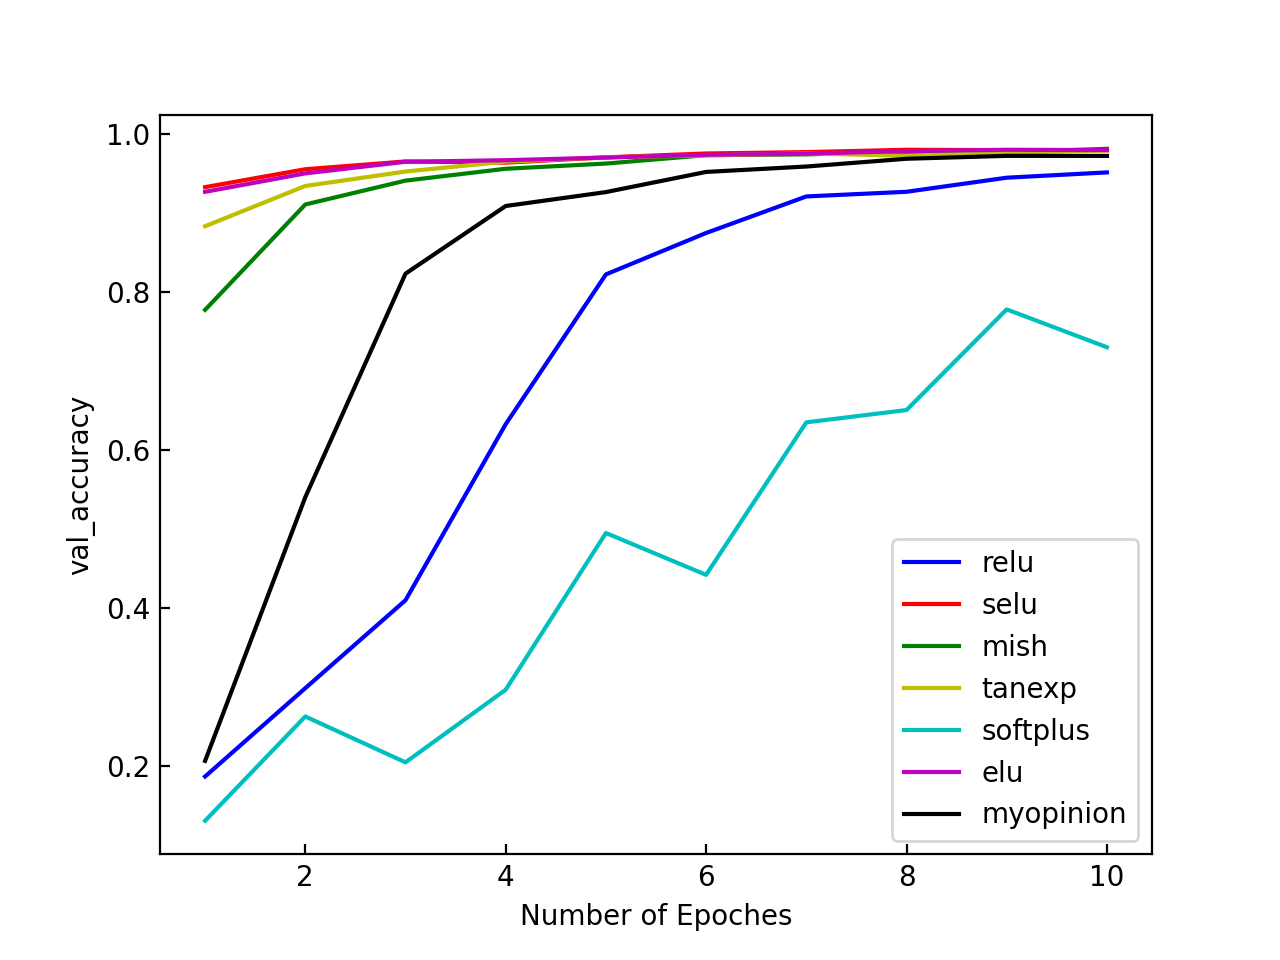
\includegraphics[width=10.0cm]{../comparison_data/mnist_val_acc.png}
    \caption{検証データでの精度}
    \label{val_acc}
  \end{center}
\end{figure}

この結果からseluは入力が大きな負の値である時に0に収束しているが、0に収束していないeluが同等の精度を出していることから入力が負の時に0に収束することが性能をよくしている訳ではないことが明確になりました。
そして、reluから定数を引いた自作関数はreluと同等の計算量にも関わらず、reluよりも早い収束を見せている結果となった。活性化関数の入力が0の時に出力も0でなければいけないという暗黙のルールに反しているが、精度が上がったため、このルールに関して触れている論文がないか調べようと考えています。

また、tanexpの論文での結果の図と比較するとreluが5エポック目から傾きが緩やかになっている点や上から三番目の活性化関数が2エポック目から傾きが緩やかになっている点など、グラフ自体は極めて近い形をしていますが、それぞれの活性化関数がグラフと対応していないように見られます。よってtanexpの論文は信頼性に劣る論文であることが検証によってわかりました。

\begin{figure}[H]
  \begin{center}
    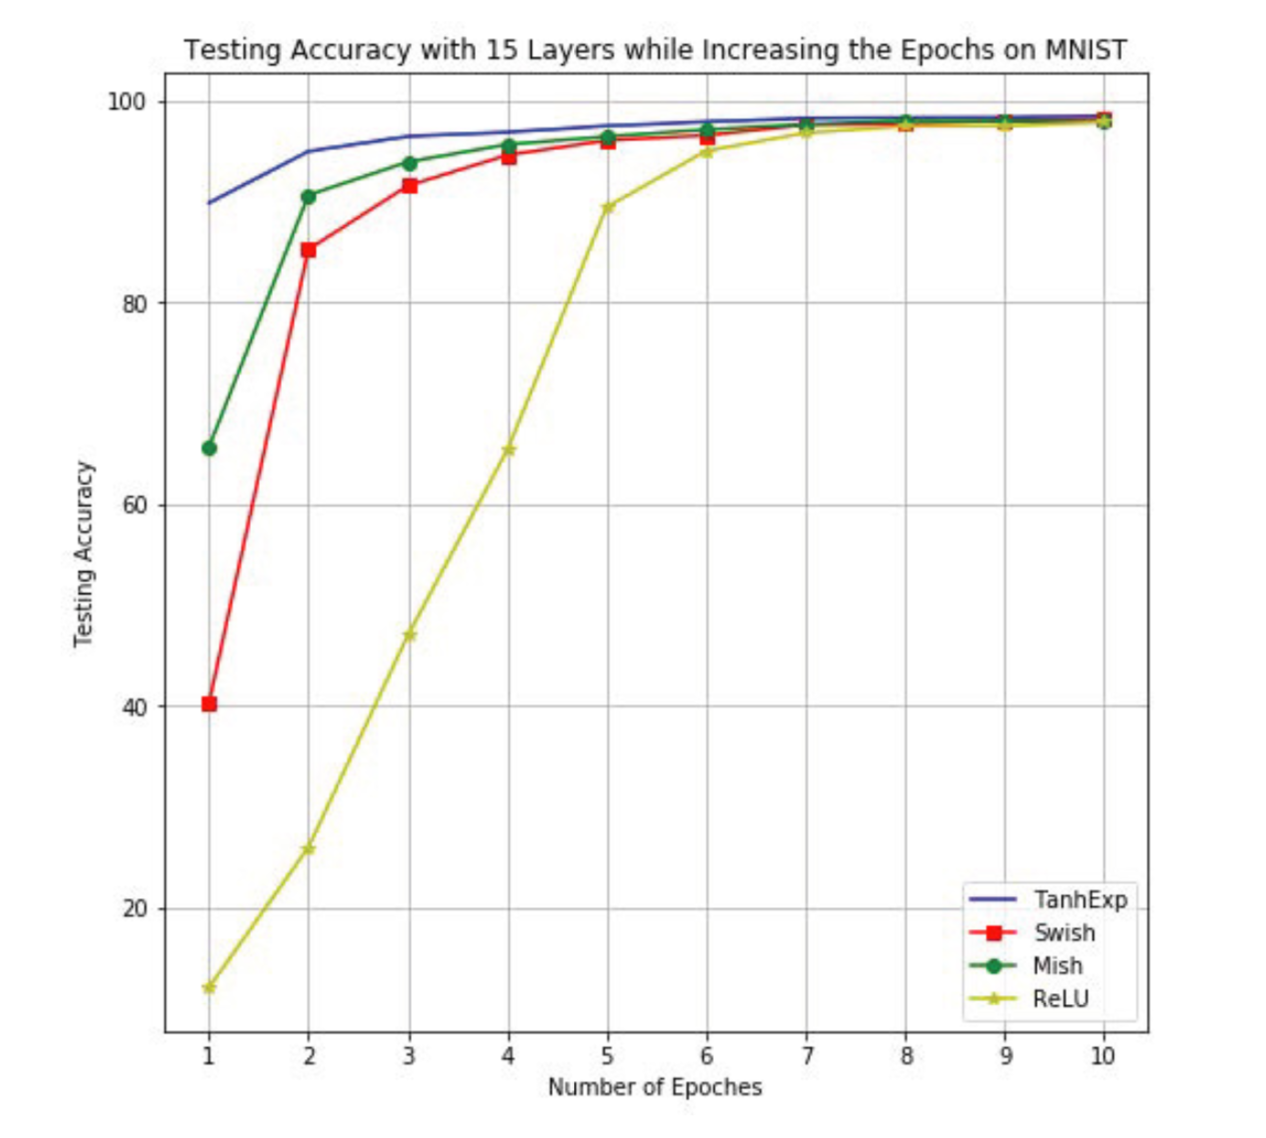
\includegraphics[width=10.0cm]{../image/tanexp_acc.png}
    \caption{tanexp論文での精度の比較結果}
    \label{tanexp_acc}
  \end{center}
\end{figure}

\section{今後の方針}
まず、tanexpの論文でも比較されている問題で、ニューラルネットワークは層を増やしすぎてしまうと精度が落ちてしまう問題があり、活性化関数によって層をどこまで増やしても精度を保つことができるか比較実験を行う予定です。ただし、今回の訓練時間の約10倍の時間がかかるため、湯川先生に勧められた論文や実装に時間を取られてしまい、まだ読めていないリプシッツ定数と活性化関数に関連する論文を読みすすめて行ければと思っています。

\end{document}
